\documentclass{beamer}
\usetheme{Darmstadt}
\usecolortheme{beaver}

% Custom colors
\definecolor{bgsubrown}{RGB}{79,44,29}
\definecolor{bgsuorange}{RGB}{253,80,0}
\setbeamercolor{structure}{fg=bgsubrown}
% \setbeamercolor{title}{fg=white}
\setbeamercolor{frametitle}{fg=bgsubrown}
\setbeamercolor{alerted text}{fg=bgsuorange}

% Add these lines to change section/subsection colors
\setbeamercolor{section in toc}{fg=bgsuorange}
\setbeamercolor{subsection in toc}{fg=bgsuorange}
\setbeamercolor{section in head/foot}{fg=bgsuorange}
\setbeamercolor{subsection in head/foot}{fg=bgsuorange}
\setbeamercolor{title}{fg=bgsuorange}

\usepackage{appendixnumberbeamer}
\setbeamertemplate{footline}[frame number]
\setbeamertemplate{navigation symbols}{}

% Additional packages
\usepackage{booktabs}
\usepackage{colortbl}
\usepackage{xcolor}
\usepackage{tikz}
\usepackage{multicol}
\usepackage{hyperref}
\usepackage{beamerappendixnote}
\usepackage{animate}

\title{Predicting Learning Commons Usage:\\Duration and Occupancy}
\subtitle{A Statistical Learning Approach}
\author{Emma Naiyue Liang, Ryan Rankin, Jaryt Salvo, \& Jason Turk}
\institute{MATH 7550 Statistical Learning | BGSU}
\date{\today}

\begin{document}

\begin{frame}
\titlepage
\end{frame}

\begin{frame}
\frametitle{Outline}
    \begin{enumerate}
        \item Exploratory Data Analysis
            \begin{itemize}
            \item Data Overview
            \item Key Patterns & Insights
            \end{itemize}
        \item Feature Engineering
            \begin{itemize}
            \item Derived Features
            \item Feature Selection
            \end{itemize}
        \item Model Building
            \begin{itemize}
            \item Model Training Overview
            \item Training Pipeline
            \item Model Evaluation Strategy
            \item Model Architecture
            \end{itemize}
        \item Evaluation
            \begin{itemize}
            \item Performance Metrics
            \item Model Comparison
            \end{itemize}
        \item Conclusions
            \begin{itemize}
            \item Key Findings
            \item Future Work
            \end{itemize}
    \end{enumerate}
\end{frame}

\section{Exploratory Data Analysis}

\begin{frame}
\frametitle{Data Overview}
    \begin{columns}
        \column{0.6\textwidth}
        \textbf{Dataset Characteristics}:
            \begin{itemize}
            \item Learning Commons visit records
            \item Train: Fall 2016 - Spring 2017
            \item Test: Fall 2017 - Spring 2018
            \item Two prediction tasks:
                \begin{itemize}
                \item Visit Duration (in minutes)
                \item Occupancy at check-in
                \end{itemize}
            \end{itemize}
            
        \textbf{Key Features}:
            \begin{itemize}
            \item Student demographics
            \item Academic performance metrics
            \item Course information
            \item Temporal visit data
            \end{itemize}
                
        \column{0.4\textwidth}
        \begin{alertblock}{Prediction Tasks}
            \begin{itemize}
            \item Part A: Predict Duration\_In\_Min
            \item Part B: Predict Occupancy (number of students present at check-in)
            \end{itemize}
        \end{alertblock}
    \end{columns}
\end{frame}

\begin{frame}
\frametitle{Data Structure \& Constraints}
    \begin{columns}
        \column{0.48\textwidth}
        \textbf{Available Features}:
            \begin{itemize}
            \item Student\_IDs
            \item Semester info
            \item Academic details
            \item Visit timing
            \item Student metrics
            \end{itemize}
            
        \column{0.48\textwidth}
        \textbf{Excluded Features}:
            \begin{itemize}
            \item Check\_Out\_Time (Task A)
            \item Duration\_In\_Min (Task B)
            \item Check\_Out\_Time (Task B)
            \end{itemize}
    \end{columns}

    \begin{block}{Data Notes}
        \begin{itemize}
        \item Visit-level granularity
        \item Multiple visits per student
        \item Class Standing may need adjustment (noted data entry issue)
        \item Predictions must be:
            \begin{itemize}
            \item Duration: Original units (minutes)
            \item Occupancy: Integer values
            \end{itemize}
        \end{itemize}
    \end{block}
\end{frame}

\begin{frame}
\frametitle{Feature Categories}
    \begin{columns}
        \column{0.48\textwidth}
        \textbf{Student Characteristics}:
            \begin{itemize}
            \item Degree Type
            \item Class Standing
            \item Major
            \item Expected Graduation
            \item Gender
            \end{itemize}
            
        \column{0.48\textwidth}
        \textbf{Academic Metrics}:
            \begin{itemize}
            \item Term Credit Hours
            \item Term GPA
            \item Total Credit Hours Earned
            \item Cumulative GPA
            \item Change in GPA
            \end{itemize}
    \end{columns}

    \begin{block}{Visit Information}
        \begin{itemize}
        \item Course details (Name, Number, Type)
        \item Semester Week (1-15)
        \item Visit timing and duration
        \end{itemize}
    \end{block}
\end{frame}

\begin{frame}
\frametitle{Key Patterns & Insights}
    \begin{columns}
        \column{0.5\textwidth}
        \textbf{Initial Findings}:
            \begin{itemize}
            \item Strong correlation between engagement and success
            \item Early warning signs identified
            \item Distinct student behavior clusters
            \end{itemize}
            
        \textbf{Data Quality}:
            \begin{itemize}
            \item Missing data patterns
            \item Outlier analysis
            \item Feature distributions
            \end{itemize}
                
        \column{0.5\textwidth}
        % Add correlation matrix or other visualization
        % \includegraphics[width=\textwidth]{path/to/correlations.png}
    \end{columns}
\end{frame}

\section{Feature Engineering}

\begin{frame}
\frametitle{Temporal Features}
    \begin{columns}[T]
        \column{0.5\textwidth}
        \textbf{Date \& Time Features}:
            \begin{itemize}
            \item Day of week
            \item Weekend flag
            \item Week of semester
            \item Month
            \item Hour of day
            \item Time categories (Morning/Afternoon/Evening)
            \end{itemize}
            
        \column{0.48\textwidth}
        \textbf{Academic Timeline}:
            \begin{itemize}
            \item Semester dates
            \item Expected graduation dates
            \item Months until graduation
            \item Week volume categories (Low/High)
            \end{itemize}
    \end{columns}

    \begin{alertblock}{Key Insight}
        Temporal patterns \textit{could} influence either duration or occupancy.
    \end{alertblock}
\end{frame}

\begin{frame}
\frametitle{Academic \& Course Features}
    \begin{columns}
        \column{0.48\textwidth}
        \textbf{Course Categorization}:
            \begin{itemize}
            \item Course level (Lower/Upper/Graduate)
            \item Course name categories
            \item Course type groupings
            \item STEM vs. Non-STEM
            \end{itemize}
            
        \column{0.48\textwidth}
        \textbf{Academic Metrics}:
            \begin{itemize}
            \item GPA categories
            \item Credit load categories
            \item Class standing (BGSU definition)
            \item Major categories
            \end{itemize}
    \end{columns}

    \begin{block}{Course Load Features}
        \begin{columns}[T]
            \column{0.5\textwidth}
            \begin{itemize}
            \item Unique courses per semester
            \item Course level mix
            \end{itemize}
            
            \column{0.48\textwidth}
            \begin{itemize}
            \item Advanced course ratio
            \item Multiple majors flag
            \end{itemize}
        \end{columns}
    \end{block}
\end{frame}

\begin{frame}
\frametitle{Visit \& Group Features}
    \begin{columns} %[T]
        \column{0.48\textwidth}
        \textbf{Visit Patterns}:
            \begin{itemize}
            \item Total visits per student
            \item Semester visits
            \item Average weekly visits
            \item Session length categories
            \end{itemize}
            
        \column{0.48\textwidth}
        \textbf{Group Dynamics}:
            \begin{itemize}
            \item Group size
            \item Group check-in flag
            \item Group size categories
                \begin{itemize}
                \item Individual
                \item Small Group (2-3)
                \item Medium Group (4-6)
                \item Large Group (7+)
                \end{itemize}
            \end{itemize}
    \end{columns}

    \begin{alertblock}{Feature Engineering Pipeline}
        Robust error handling and column validation for each transformation across both \texttt{LC\_train} and \texttt{LC\_test} datasets.
    \end{alertblock}
\end{frame}

\begin{frame}
\frametitle{Feature Categories Overview}
    \begin{center}
    \small
    \begin{tabular}{>{\columncolor{bgsubrown!20}}l l}
    \toprule
    \textbf{Category} & \textbf{Key Features} \\
    \midrule
    Temporal & Time of day, Day of week, Week of semester \\
    \midrule
    Academic & Course level, GPA categories, Credit load \\
    \midrule
    Visit & Duration patterns, Group sizes, Visit frequency \\
    \midrule
    Course & Subject areas, Level progression, Course mix \\
    \midrule
    Student & Major groups, Class standing, Academic progress \\
    \bottomrule
    \end{tabular}
    \end{center}

    \begin{alertblock}{Engineering Approach}
        \vspace{-0.2cm}
        \begin{columns}
            \column{0.48\textwidth}
            \begin{itemize}
            \item Temporal patterns
            \item Academic context
            \end{itemize}
            
            \column{0.48\textwidth}
            \begin{itemize}
            \item Student behavior
            \item Group dynamics
            \end{itemize}
        \end{columns}
    \end{alertblock}
\end{frame}

\section{Model Building}

\begin{frame}
\frametitle{Training Pipeline}
    \noindent\centering
    \hspace{-0.6cm}
    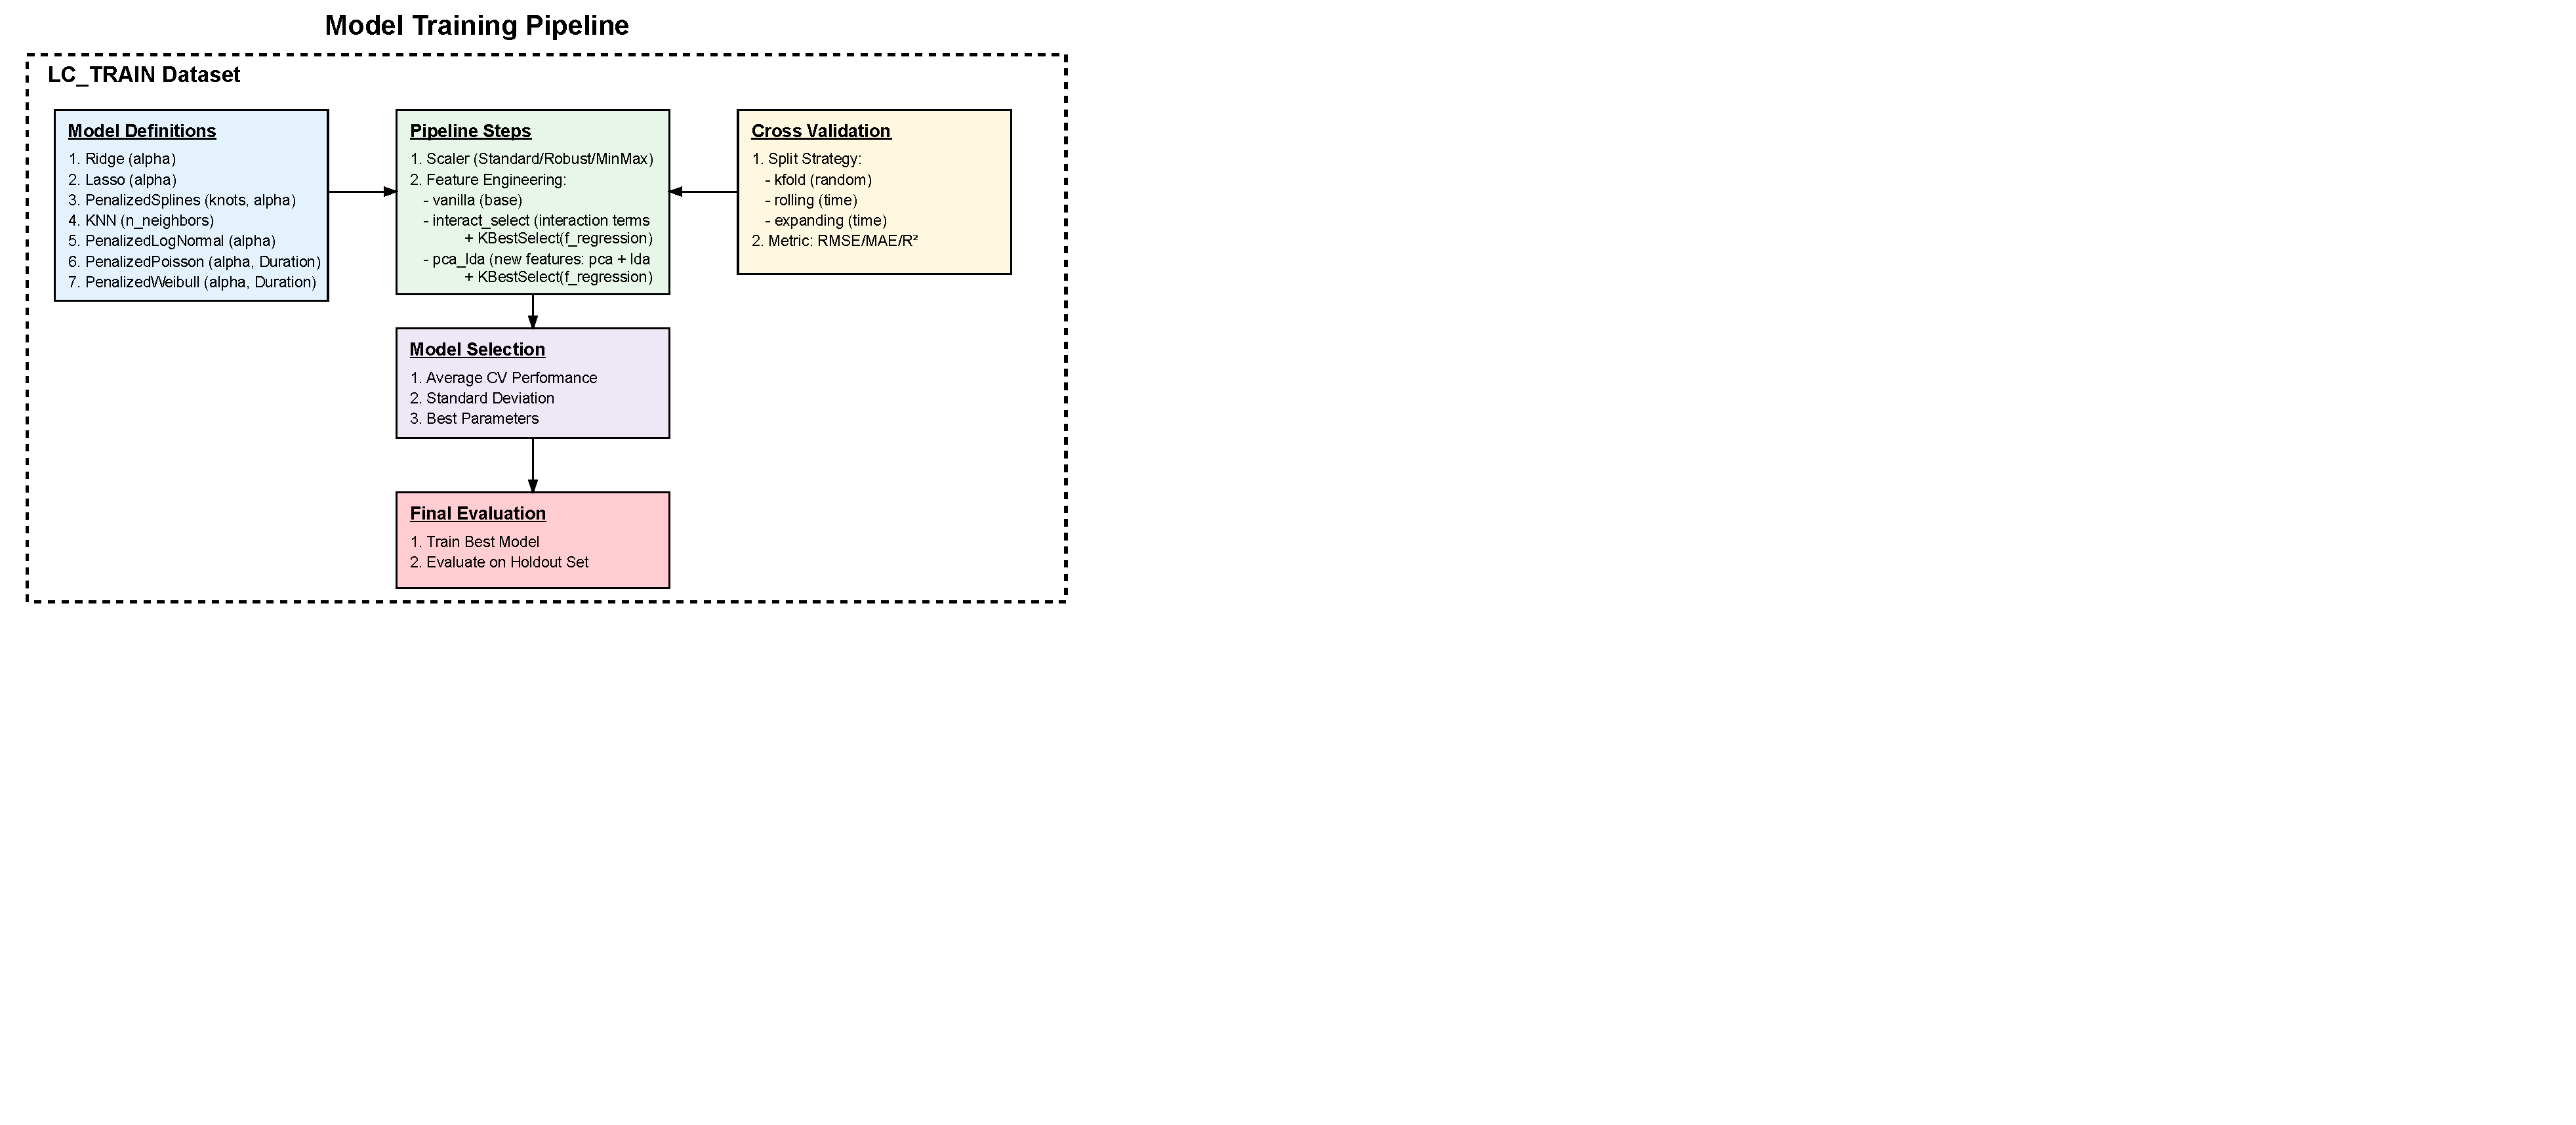
\includegraphics[width=1.1\textwidth, height=0.9\textheight,
        % keepaspectratio,    % Maintains aspect ratio
        interpolate=false,  % Prevents blurry interpolation
        draft=false]{images/modeling/data_flow.pdf}
\end{frame}
    
\begin{frame}
\frametitle{Model Training Overview}
    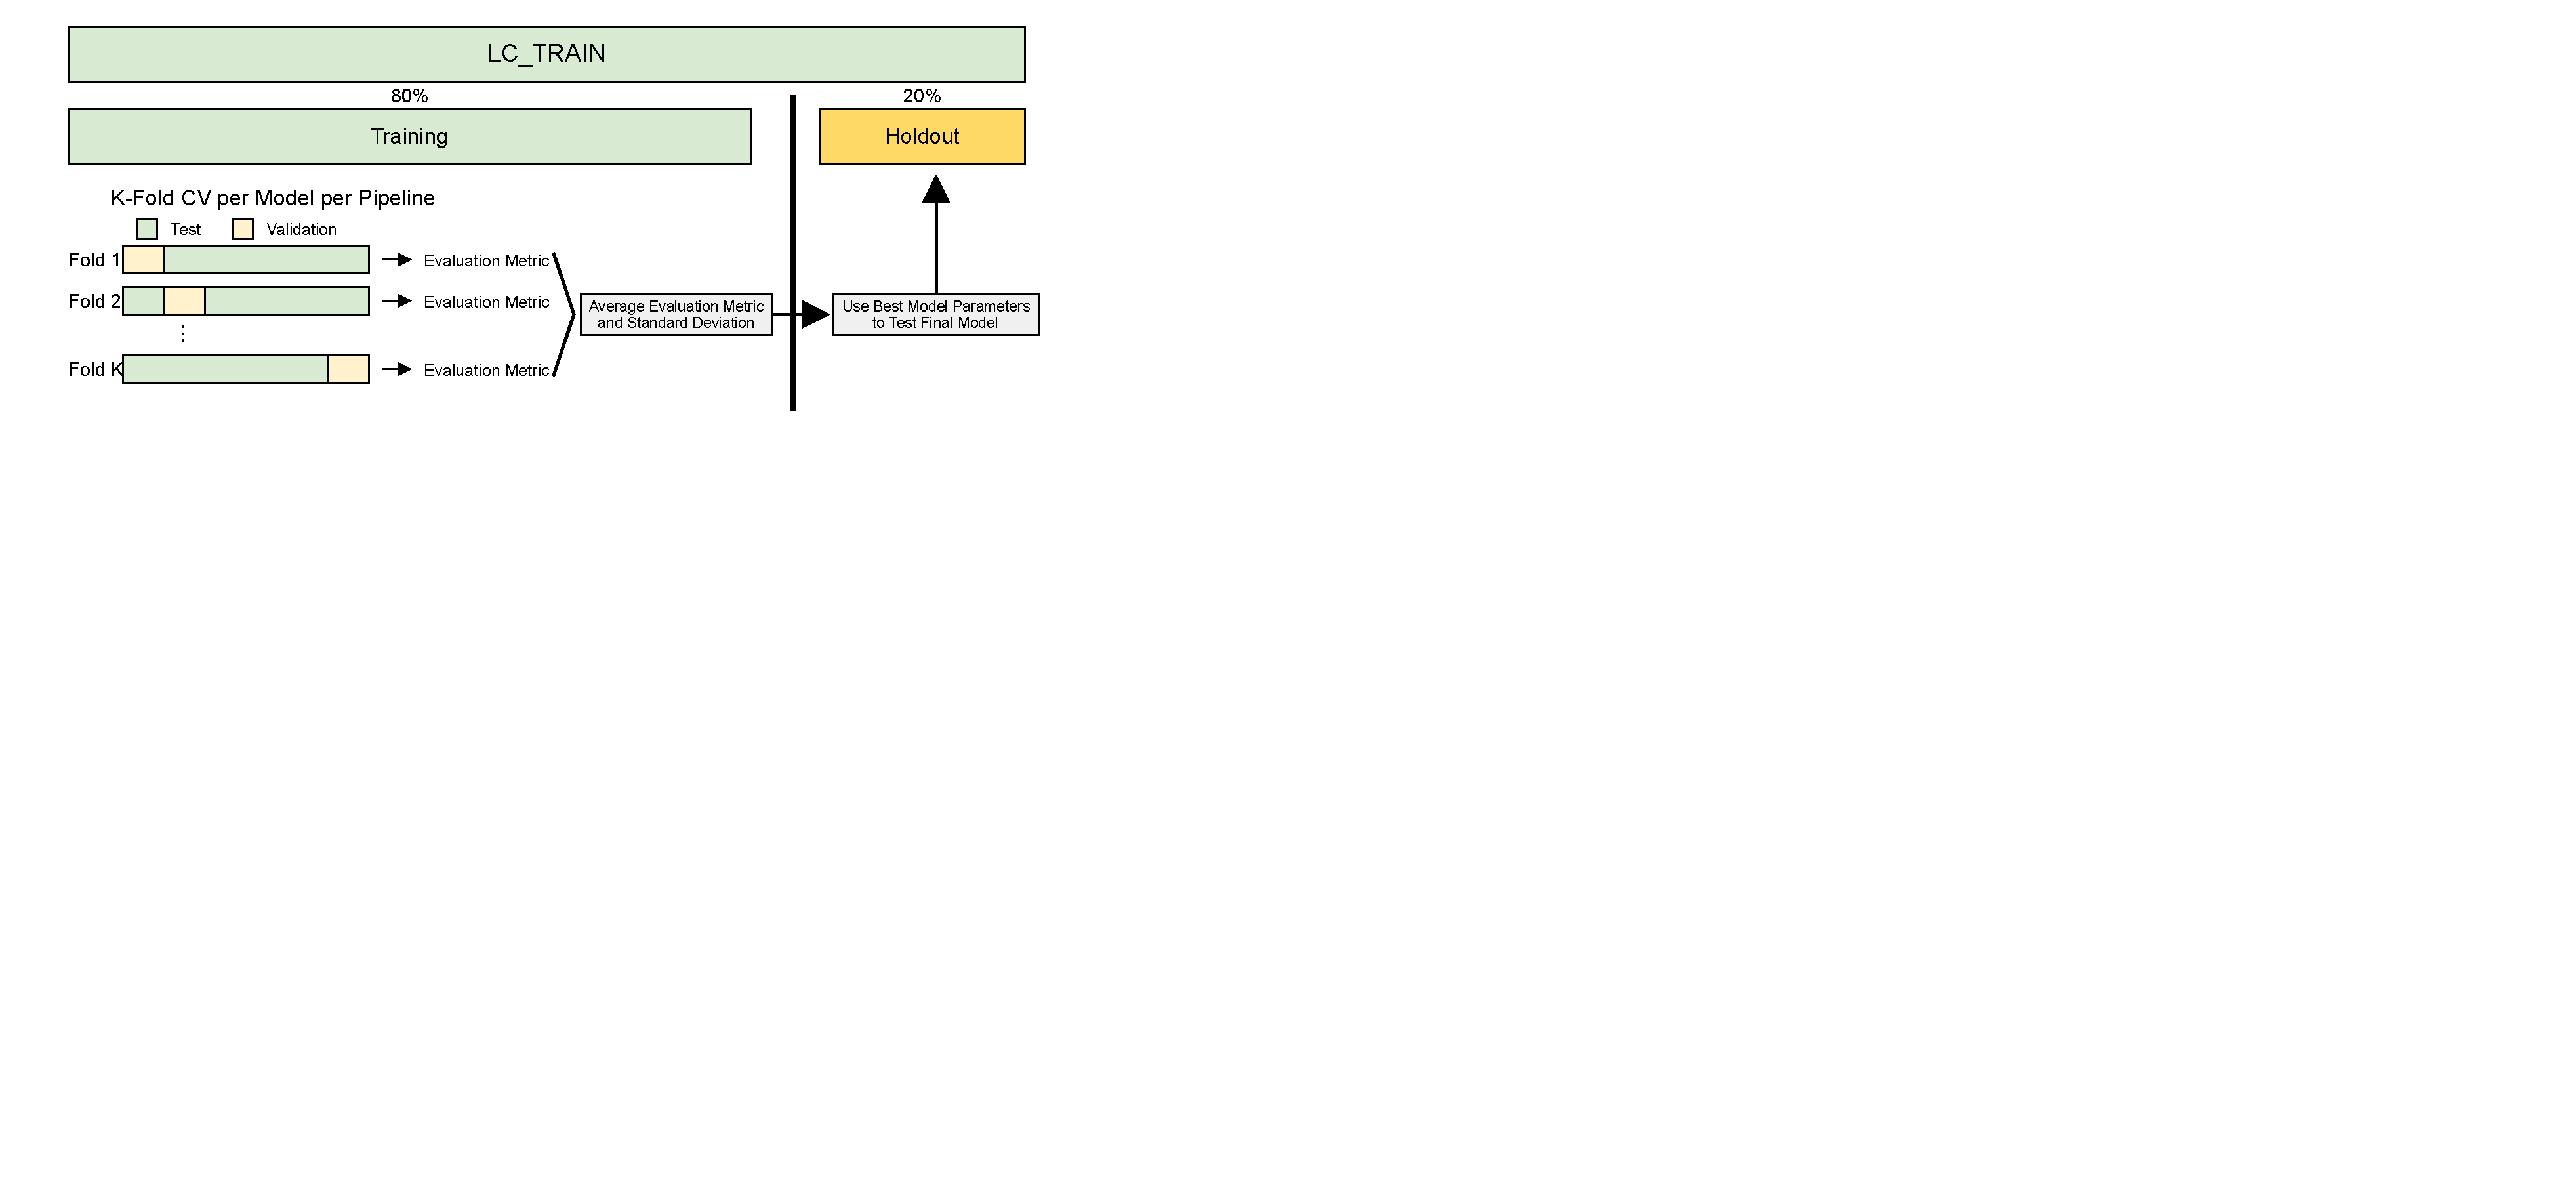
\includegraphics[width=\textwidth]{images/modeling/model_building.pdf}
    
    \begin{alertblock}{Key Points}
        \begin{columns}[T,onlytextwidth]
            \column{0.5\textwidth}
            \begin{itemize}
            \item Model pipeline combines:
                \begin{itemize}
                \item Multiple model types
                \item Feature engineering steps
                \item Cross-validation strategies
                \end{itemize}
            \end{itemize}
            
            \column{0.5\textwidth}
            \begin{itemize}
            \item Training approach:
                \begin{itemize}
                \item 80/20 train-holdout split
                \item CV metrics: RMSE \& R²
                \item Best model via avg performance
                \end{itemize}
            \end{itemize}
        \end{columns}
    \end{alertblock}
\end{frame}

\begin{frame}
\frametitle{Model Evaluation Strategy}
    \begin{columns} % [T] aligns columns at the top
        \column{0.48\textwidth}
        \textbf{Training \& Validation}:
            \begin{itemize}
            \item Cross-validation strategy
                \begin{itemize}
                \item Time-based splits
                \item Grid search optimization
                \end{itemize}
            \item Performance monitoring
                \begin{itemize}
                \item Consistent metrics
                \item Error analysis
                \end{itemize}
            \end{itemize}
            
        \column{0.48\textwidth}
        \textbf{Testing \& Deployment}:
            \begin{itemize}
            \item Hold-out evaluation
                \begin{itemize}
                \item RMSE \& MAE metrics
                \item R² assessment
                \item Diagnostic plots
                \end{itemize}
            \item Model monitoring
                \begin{itemize}
                \item Performance tracking
                \end{itemize}
            \end{itemize}
    \end{columns}

    \begin{alertblock}{MLflow Pipeline Integration}
        \begin{columns}[T]
            \column{0.48\textwidth}
            \begin{itemize}
            \item Experiment tracking
            \item Automated logging
            \end{itemize}
            
            \column{0.48\textwidth}
            \begin{itemize}
            \item Parameter logging
            \item Model versioning
            \end{itemize}
        \end{columns}
    \end{alertblock}
\end{frame}

\begin{frame}
\frametitle{Model Architecture}
    \begin{center}
    \small
    \begin{tabular}{>{\columncolor{bgsubrown!20}}l l}
    \toprule
    \textbf{Component} & \textbf{Implementation} \\
    \midrule
    Pipeline & Feature selection $\rightarrow$ Scaling $\rightarrow$ Model \\
    \midrule
    Cross-validation & Time-based split with multiple methods \\
    \midrule
    Hyperparameters & Grid search with parallel processing (\texttt{joblib}) \\
    \midrule
    Error Metrics & RMSE (primary), R² (secondary) \\
    \midrule
    Output & Model artifacts + performance metrics \\
    \bottomrule
    \end{tabular}
    \end{center}

    \begin{block}{Implementation Details}
        \begin{itemize}
        \item Separate experiment tracking for each task
        \item Robust error handling and logging
        \item Automated model registration
        \item Comprehensive results storage
        \end{itemize}
    \end{block}
\end{frame}

\section{Evaluation}

\begin{frame}
\frametitle{Duration: Performance on Holdout Set}
    \begin{columns}
        \column{0.5\textwidth}
        \begin{center}
        \small
        \begin{tabular}{>{\columncolor{bgsubrown!20}}l r r}
        \toprule
        \textbf{CV Method} & \textbf{RMSE} & \textbf{R²} \\
        \midrule
        expanding & 60.41 & 0.029 \\
        rolling & 60.45 & 0.028 \\
        kfold & 60.51 & 0.026 \\
        \bottomrule
        \end{tabular}
        \end{center}
            
        \column{0.5\textwidth}
        \begin{center}
        \small
        \begin{tabular}{>{\columncolor{bgsubrown!20}}l r r}
        \toprule
        \textbf{Pipeline} & \textbf{RMSE} & \textbf{R²} \\
        \midrule
        vanilla & 60.20 & 0.035 \\
        interact\_select & 60.55 & 0.024 \\
        pca\_lda & 60.61 & 0.022 \\
        \bottomrule
        \end{tabular}
        \end{center}
    \end{columns}

    \vspace{0.2cm}
    \begin{center}
    \small
    \begin{tabular}{>{\columncolor{bgsubrown!20}}l r r r r}
    \toprule
    \textbf{Model} & \textbf{RMSE} & \textbf{(std)} & \textbf{R²} & \textbf{(std)} \\
    \midrule
    PenalizedSplines & 60.03 & $\pm$ 0.63 & 0.041 & $\pm$ 0.020 \\
    Ridge & 60.39 & $\pm$ 0.17 & 0.030 & $\pm$ 0.005 \\
    PenalizedLogNormal & 60.49 & $\pm$ 0.15 & 0.026 & $\pm$ 0.005 \\
    Lasso & 60.50 & $\pm$ 0.28 & 0.026 & $\pm$ 0.009 \\
    KNN & 60.85 & $\pm$ 0.54 & 0.014 & $\pm$ 0.018 \\
    \bottomrule
    \end{tabular}
    \end{center}
    
    \vspace{-0.2cm}
    \begin{alertblock}{Key Insight}
        Above tables are aggregates. PenalizedSplines with vanilla features and KFold CV achieved best performance on holdout set.
    \end{alertblock}
\end{frame}

\begin{frame}
\frametitle{Duration: Best Model Diagnostics}
    \begin{center}
        \noindent\centering
        \vspace{-0.7cm}
        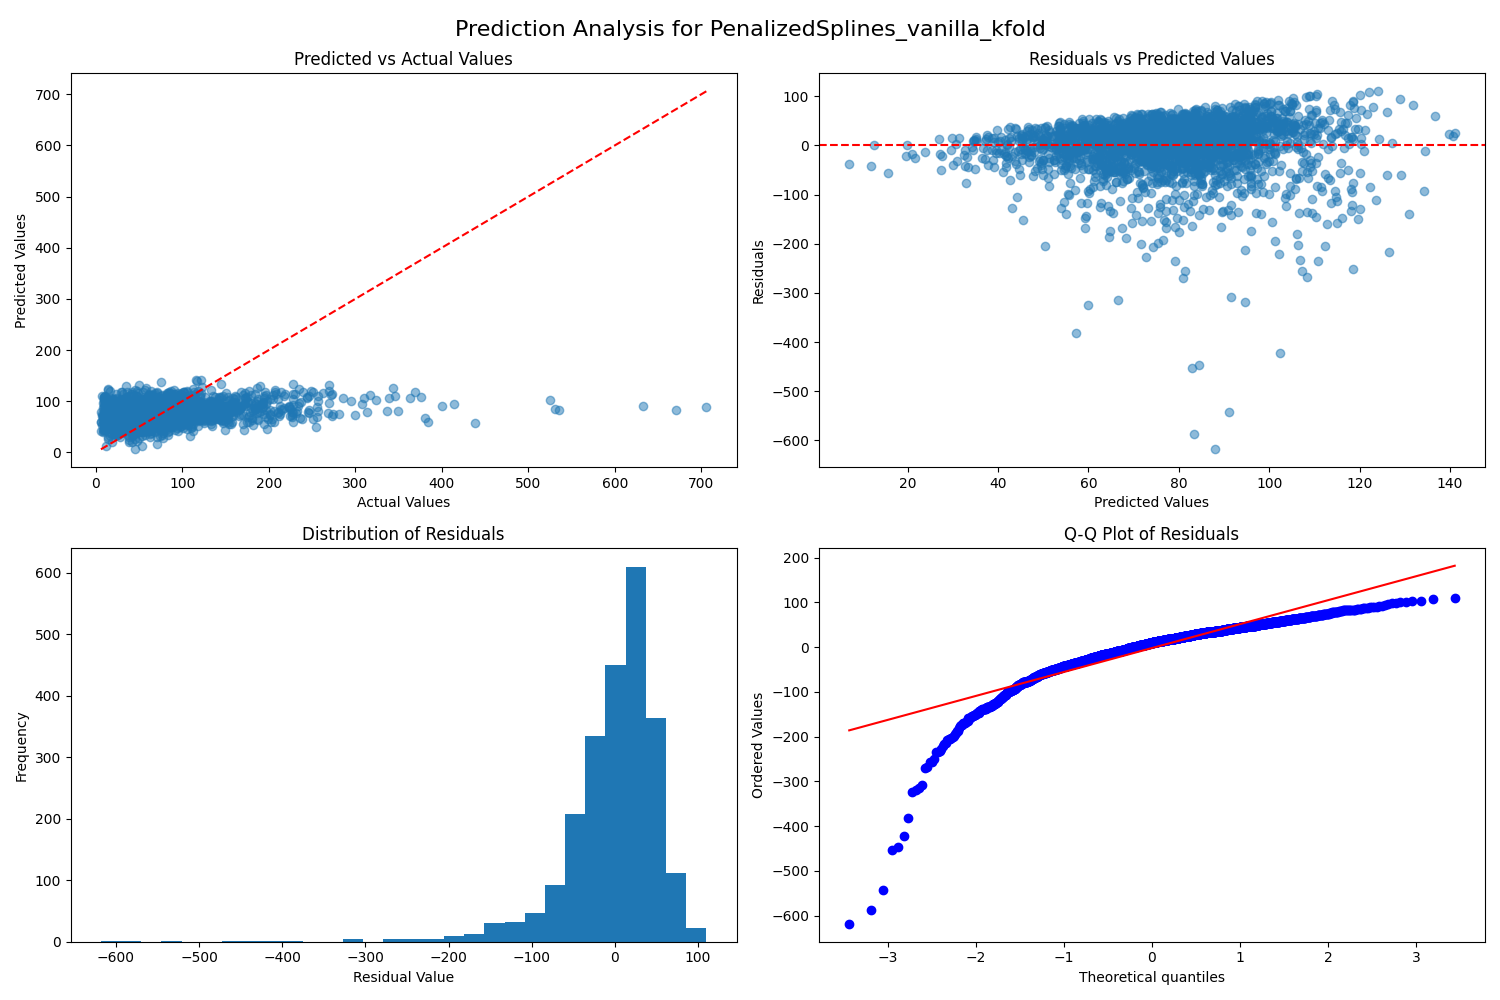
\includegraphics[width=1.0\textwidth, height=0.95\textheight,
            % keepaspectratio,    % Maintains aspect ratio
            interpolate=false,  % Prevents blurry interpolation
            draft=false]{images/evaluation/Duration_PenalizedSplines_vanilla_kfold.jpg}
    \end{center}
\end{frame}

\begin{frame}
    \frametitle{Occupancy: Performance on Holdout Set}
        \begin{columns}
            \column{0.5\textwidth}
            \begin{center}
            \small
            \begin{tabular}{>{\columncolor{bgsubrown!20}}l r r}
            \toprule
            \textbf{CV Method} & \textbf{RMSE} & \textbf{R²} \\
            \midrule
            expanding & 4.32 & 0.000 \\
            rolling & 4.34 & -0.021 \\
            kfold & 4.59 & -0.156 \\
            \bottomrule
            \end{tabular}
            \end{center}
                
            \column{0.5\textwidth}
            \begin{center}
            \small
            \begin{tabular}{>{\columncolor{bgsubrown!20}}l r r}
            \toprule
            \textbf{Pipeline} & \textbf{RMSE} & \textbf{R²} \\
            \midrule
            vanilla & 4.04 & 0.138 \\
            interact\_select & 4.45 & -0.052 \\
            pca\_lda & 4.76 & -0.263 \\
            \bottomrule
            \end{tabular}
            \end{center}
        \end{columns}
    
        \vspace{0.2cm}
        \begin{center}
        \small
        \begin{tabular}{>{\columncolor{bgsubrown!20}}l r r r r}
        \toprule
        \textbf{Model} & \textbf{RMSE} & \textbf{(std)} & \textbf{R²} & \textbf{(std)} \\
        \midrule
        PenalizedSplines & 4.00 & $\pm$ 0.50 & 0.150 & $\pm$ 0.231 \\
        PenalizedWeibull & 4.04 & $\pm$ 0.14 & 0.141 & $\pm$ 0.059 \\
        Lasso & 4.17 & $\pm$ 0.24 & 0.084 & $\pm$ 0.103 \\
        PenalizedPoisson & 4.17 & $\pm$ 0.24 & 0.082 & $\pm$ 0.110 \\
        Ridge & 4.61 & $\pm$ 0.62 & -0.136 & $\pm$ 0.311 \\
        KNN & 5.51 & $\pm$ 1.29 & -0.675 & $\pm$ 0.829 \\
        \bottomrule
        \end{tabular}
        \end{center}
        
        \vspace{-0.2cm}
        \begin{alertblock}{Key Insight}
            Also aggregates. Vanilla \textit{rolling} PenalizedSplines proved best.
        \end{alertblock}
    \end{frame}

\begin{frame}
\frametitle{Occupancy: Best Model Diagnostics}
    \begin{center}
        \noindent\centering
        \vspace{-0.7cm}
        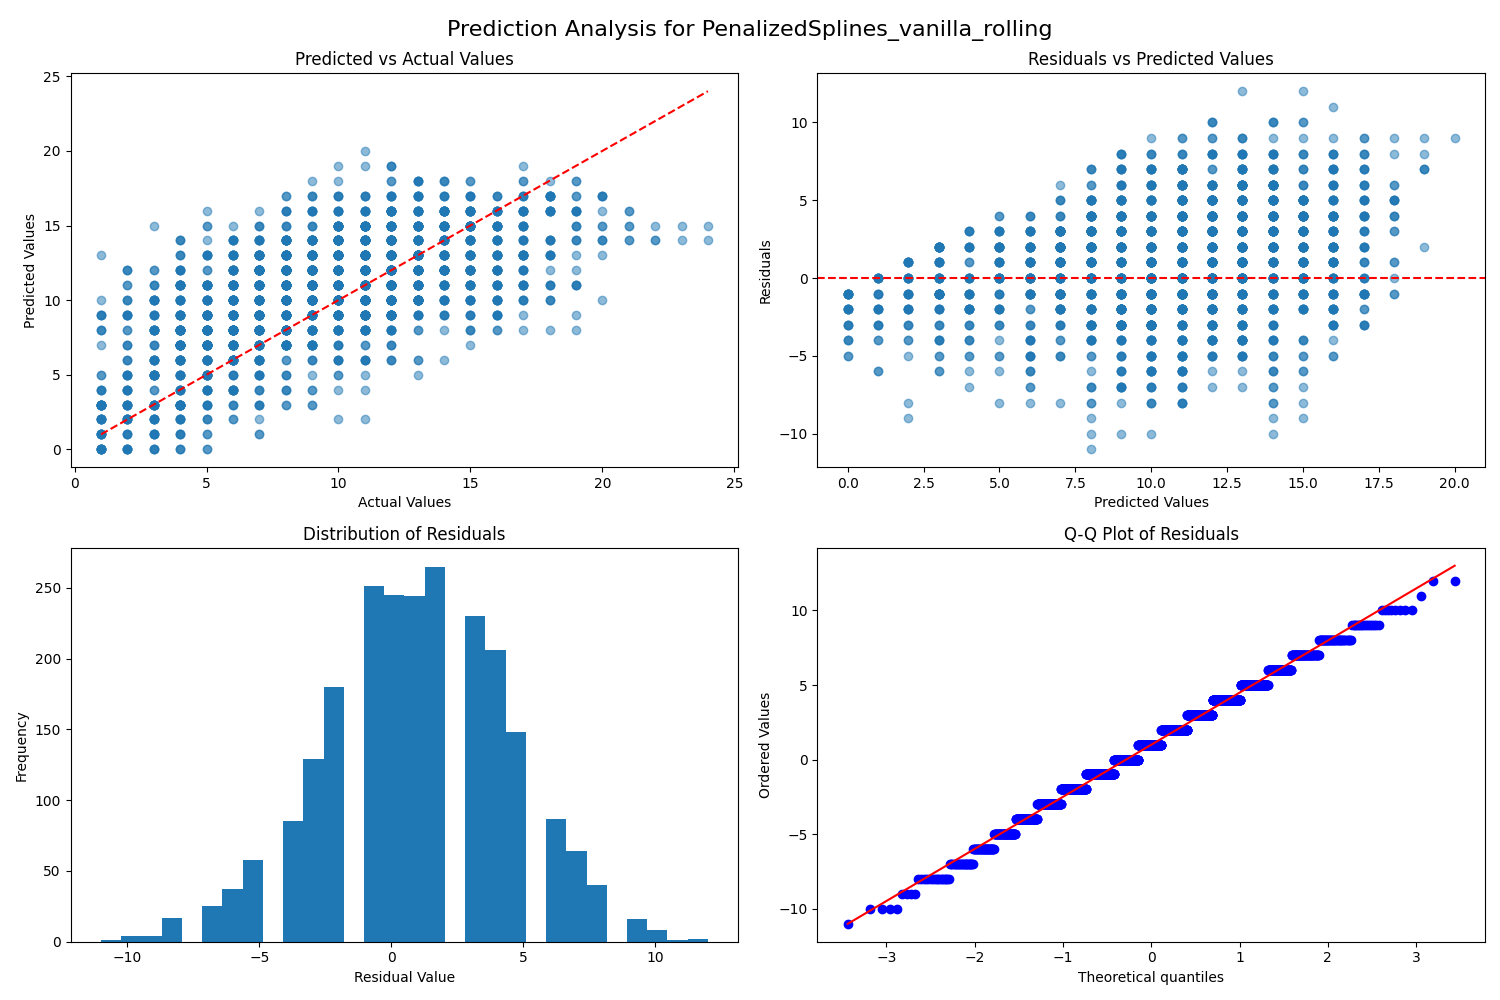
\includegraphics[width=1.0\textwidth, height=0.95\textheight,
            % keepaspectratio,    % Maintains aspect ratio
            interpolate=false,  % Prevents blurry interpolation
            draft=false]{images/evaluation/Occupancy_PenalizedSplines_vanilla_rolling.jpg}
    \end{center}
\end{frame}

\begin{frame}
    \frametitle{Best Model Configurations}
        \begin{columns}[T]
            \column{0.48\textwidth}
            \textbf{Duration Prediction}:
            \vspace{-0.5cm}
            \begin{center}
            \small
            \begin{tabular}{>{\columncolor{bgsubrown!20}}l l}
            \toprule
            \textbf{Component} & \textbf{Value} \\
            \midrule
            Model & PenalizedSplines \\
            Pipeline & vanilla \\
            CV Method & kfold \\
            RMSE & 59.47 \\
            R² & 0.059 \\
            \midrule
            Ridge $\alpha$ & 14.38 \\
            Spline degree & 3 \\
            Spline knots & 15 \\
            Scaler & RobustScaler \\
            \bottomrule
            \end{tabular}
            \end{center}
                
            \column{0.48\textwidth}
            \textbf{Occupancy Prediction}:
            \vspace{-0.5cm}
            \begin{center}
            \small
            \begin{tabular}{>{\columncolor{bgsubrown!20}}l l}
            \toprule
            \textbf{Component} & \textbf{Value} \\
            \midrule
            Model & PenalizedSplines \\
            Pipeline & vanilla \\
            CV Method & rolling \\
            RMSE & 3.64 \\
            R² & 0.303 \\
            \midrule
            Ridge $\alpha$ & 29.76 \\
            Spline degree & 3 \\
            Spline knots & 15 \\
            Scaler & RobustScaler \\
            \bottomrule
            \end{tabular}
            \end{center}
        \end{columns}
    
        \begin{alertblock}{Key Insight}
            Both tasks achieved best results with PenalizedSplines and vanilla features, though with different CV methods \& regularization.
        \end{alertblock}
    \end{frame}

\section{Conclusion}

\begin{frame}
\frametitle{Key Findings}
    \begin{columns}
        \column{0.6\textwidth}
        \textbf{Main Results}:
            \begin{itemize}
            \item Early prediction possible (Week 3)
            \item Strong predictive features identified
            \item Model generalizes well across courses
            \end{itemize}
            
        \textbf{Future Work}:
            \begin{itemize}
            \item Real-time prediction system
            \item Additional data sources
            \item Intervention strategies
            \item Model interpretability
            \end{itemize}
                
        \column{0.4\textwidth}
        % Add final summary visualization
        % \includegraphics[width=\textwidth]{path/to/summary.png}
    \end{columns}

    \begin{alertblock}{Impact}
        System enables early identification of at-risk students for timely intervention
    \end{alertblock}
\end{frame}

\end{document} 